\documentclass[table]{beamer}

% Customize slide appearance
\mode<presentation>
{
  \usetheme{Warsaw}
  \setbeamercovered{transparent}
}

\usepackage[english]{babel}
\usepackage{times}
\usefonttheme[onlymath]{serif} 
\setbeamertemplate{navigation symbols}{}

% You can add any graphics to every slide by following command:
% \logo{\resizebox{0.1\textwidth}{!}{\includegraphics{col_small}}}
% \logo{\resizebox{0.2\textwidth}{!}{
\includegraphics{imperialblue}}}

% Uncomment this, if you want the table of contents before each subsection.
% However, to edit slides in TeXWord avoiding this feature is good idea.
% \AtBeginSubsection[]
% {
%   \begin{frame}<beamer>
%     \frametitle{Outline}
%     \tableofcontents[currentsection,currentsubsection]
%   \end{frame}
% }

% If you wish to uncover everything in a step-wise fashion, uncomment
% the following command: 
%\beamerdefaultoverlayspecification{<+->}
\xdefinecolor{keyword}{rgb}{0,0,1}
\xdefinecolor{ctext}{rgb}{0.64,0.08,0.08}
\xdefinecolor{cline}{rgb}{0.17,0.57,0.69}
\xdefinecolor{comment}{rgb}{0,0.5,0.0}
\newif\ifschigh\schighfalse
\newcommand{\kw}[1]{\ifschigh\textcolor{red}{#1}\else\textcolor{keyword}{#1}\fi}
\newcommand{\kt}[1]{\ifschigh\textcolor{red}{#1}\else\textcolor{ctext}{#1}\fi}
\newcommand{\kc}[1]{\ifschigh\textcolor{red}{#1}\else\textcolor{comment}{#1}\fi}
\addtobeamertemplate{alerted text begin}{\global\schightrue%
}{}
\defbeamertemplate*{alerted text end}{default}{\global\schighfalse%
}



\newcounter{sckll}
\newcommand{\kr}{\setcounter{sckll}{1}}
\newcommand{\krr}[1]{\setcounter{sckll}{#1}}
\newcommand{\klvalue}{\ifnum\value{sckll}<10{\hphantom{0}}\fi\arabic{sckll}\addtocounter{sckll}{1}}
%\newcommand{\kl}{\ifschigh\textcolor{red}{\klvalue}\else\textcolor{cline}{\klvalue}\fi\hspace{2ex}}
\newcommand{\kl}{}

\let\oldurl=\url
\renewcommand{\url}[1]{\textcolor{blue}{\oldurl{#1}}}

\usepackage{tikz, pgfbaseplot, pgflibrarysnakes,pgflibraryarrows}

\begin{document}

% Title Data. We keep it after \begin{document} 
% to enable editing text in BaKoMa TeX Word.

\title[C for Science - Lecture 2]{Computing in C for Science}
\subtitle{Lecture 2 of 5}

% Use the \inst command to identify several affiliations.
\author[Steven Capper]{Dr. Steven Capper \\ {\tt steven.capper99@imperial.ac.uk}\\
\url{http://www2.imperial.ac.uk/~sdc99/ccourse/}}

\date{$23^\text{rd}$ November 2011 }

\subject{C for Science} % Should be passed to PDF [YNI]
{
\logo{
\includegraphics[width=0.30\textwidth]{imperialblue}}
\begin{frame}
  \titlepage
\end{frame}
}

\begin{frame}
\frametitle{Preprocessor Directives}
\begin{itemize}
\item One example is:
\begin{center}
\tt \kw{\#include} \kt{<stdio.h>}
\end{center}
Which tells the compiler to search \kt{\tt <stdio.h>} for functions.
\item Another example is:
\begin{center}
\tt \kw{\#define} MAXSIZE 1024
\end{center}
This replaces all occurrences of {\tt MAXSIZE} with {\tt 1024}.
\begin{itemize}
\item Define statements can be named in a similar way to variables, but
\item It is convention to use upper case for \kw{\tt \#define} statements.
\end{itemize}
\item Or even simpler:
\begin{center}
\tt \kw{\#define} NDEBUG
\end{center}
Meaning {\tt NDEBUG} is defined. This will be expanded later on.
\end{itemize}
\end{frame}

\begin{frame}
\frametitle{Functions with Variable Number of Arguments}
Sometimes we don't know in advance how many arguments (or what type) a function needs, so C allows functions to have an unknown number of arguments. Two examples we've seen so far are {\tt printf} and {\tt scanf}.

\begin{itemize}
\item The first parameter must be of a normal type (i.e. \kw{\tt int}).
\item Three dots ({\tt ...}) are used for the last parameter.
\end{itemize}
\begin{center}
{\tt \kw{int} printf(\kw{char} * formatString, ...)}
\end{center}
\begin{block}{Handling variable arguments}
Variable arguments are manipulated using {\tt va\_start()}, {\tt va\_arg()},
and {\tt va\_end()}. These are found in \kt{\tt <stdarg.h>}.
\end{block}

\begin{alertblock}{}
Having just introduced these, I'm going to ask you {\bf not} to use them! Arrays are almost always more appropriate to use.
\end{alertblock}
\end{frame}

\begin{frame}[fragile]
\frametitle{The Stack}
Let's consider this example function.
\begin{columns}
\begin{column}{5cm}
\begin{semiverbatim}
\kw{int} hasRealRoots(\alert<2>{\kw{double} A},
       \alert<2>{\kw{double} B, \kw{double} C})
\{
   \alert<3>{\kw{double} d} = B*B-4.0*A*C;
   \kw{if} (d < 0) \alert<4>{\kw{return}} 0;
   \alert<4>{\kw{return}} 1;
\}
\end{semiverbatim}
\end{column}
\begin{column}{5cm}
\begin{itemize}
\alert<2>{\item We need space to hold a copy of {\tt A}, {\tt B} and {\tt C}.} 
\alert<3>{\item We need space to store our computed {\tt d}.}
\alert<4>{\item When we've finished, we need to get back to the calling function.}
\end{itemize}
\end{column}
\end{columns}
\vspace{0.1in}
\begin{block}<5>{}
\begin{center}
\alert<5>{This is achieved by using a \emph{stack}.}
\end{center}
\end{block}
\end{frame}

\begin{frame}
\frametitle{The Stack - Rough Sketch (Stack Frames)}

\begin{columns}
\begin{column}{5cm}
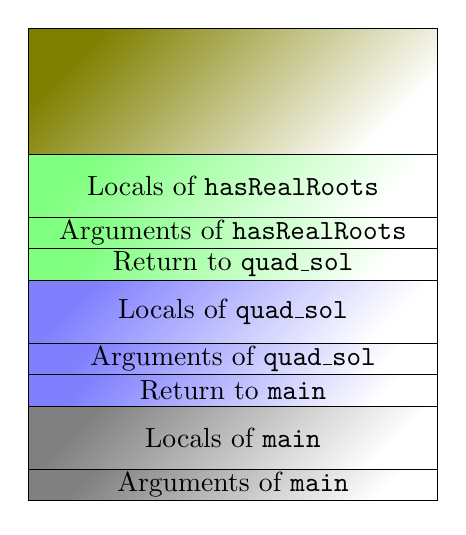
\begin{tikzpicture}[]
\shadedraw [shading angle=45] (0,0) rectangle +(5.2,0.4);
\node at (2.6,0.2) {Arguments of \tt main};
\shadedraw [shading angle=45] (0,0.4) rectangle +(5.2,0.8);
\node at (2.6,0.8) {Locals of \tt main};
\shadedraw [top color=blue!50,shading angle=45] (0,1.2) rectangle +(5.2,0.4);
\node at (2.6,1.4) {Return to \tt main};
\shadedraw [top color=blue!50,shading angle=45] (0,1.6) rectangle +(5.2,0.4);
\node at (2.6,1.8) {Arguments of \tt quad\_sol};
\shadedraw [top color=blue!50,shading angle=45] (0,2.0) rectangle +(5.2,0.8);
\node at (2.6,2.4) {Locals of \tt quad\_sol};
\shadedraw [top color=green!50,shading angle=45] (0,2.8) rectangle +(5.2,0.4);
\node at (2.6,3.0) {Return to \tt quad\_sol};
\shadedraw [top color=green!50,shading angle=45] (0,3.2) rectangle +(5.2,0.4);
\node at (2.6,3.4) {Arguments of \tt hasRealRoots};
\shadedraw [top color=green!50,shading angle=45] (0,3.6) rectangle +(5.2,0.8);
\node at (2.6,4.0) {Locals of \tt hasRealRoots};
\shadedraw [top color=green!50!red,shading angle=45] (0,4.4) rectangle +(5.2,1.6);
\end{tikzpicture}
\end{column}
\begin{column}{6cm}
\begin{itemize}
\item Consider the case where we have {\tt main}, which calls \textcolor{blue}{\tt quad\_sol}, which in turn calls \textcolor{green}{\tt hasRealRoots}.
\item We add and remove items from the stack as the program executes.
\item Adding/removing items from the stack takes very little time.
\item The stack is fixed in size, if we go over the top (``smash the stack'')
, our program crashes.
\end{itemize}
\end{column}
\end{columns}
\end{frame}

\begin{frame}
\frametitle{Recursive Functions}
As C uses a stack by default when calling functions, we are able to write functions that call themselves. These are called \emph{recursive functions}.

\begin{block}{An Example: Computing the Factorial}
$$n! = \prod_{i=1}^n i,  \quad 0! = 1, \qquad n\in\mathbb{N}.$$
Lends itself to be coded up as a recursive function.
\end{block}

\begin{block}{A Tougher Example: Fibonacci Numbers}
$$ F_n = F_{n-1} + F_{n-2}, \qquad F_0 = F_1 = 1.$$
A na\"ive implementation of this will kill the stack, and take a very long time to execute.
\end{block}
\end{frame}

\begin{frame}[fragile]
\frametitle{Computing the Factorial}
\begin{semiverbatim}
\kr\kl\kw{\#include} \kt{<stdio.h>}
\kl
\kl\kw{int} NFact(\kw{int} N)
\kl\{
\kl   \kw{if} (N>1) \kw{return} N*NFact(N-1);
\kl   \kw{return} 1;
\kl\}
\kl
\kl\kw{int} main()
\kl\{
\kl   \kw{int} n;
\kl   printf(\kt{"Enter n:"});
\kl   scanf(\kt{"%d"}, &n);
\kl   printf(\kt{"%d! = %d\\n"}, n, NFact(n));
\kl   \kw{return} 0;
\kl\}
\end{semiverbatim}
\end{frame}

\begin{frame}[fragile]
\frametitle{Computing Fibonacci Numbers}
\begin{columns}
\begin{column}{6cm}
\begin{alertblock}{}
\begin{semiverbatim}
\kw{int} BadFib(\kw{int} N)
\{
   \kw{if} (N < 2) \kw{return} 1;
   \kw{return} (BadFib(N-1) +
           BadFib(N-2));
\}
\end{semiverbatim}
\end{alertblock}
\end{column}
\begin{column}{3cm}
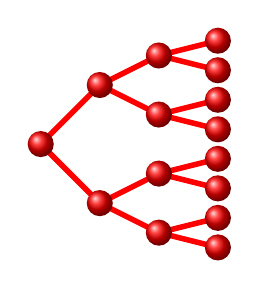
\begin{tikzpicture}[scale=0.75]
\tikzstyle{every node}=[ball color=red,circle,text=white]
\tikzstyle{edge from parent}=[draw,dashed,thick,red]
\draw[line width=2pt,color=red] (0,0) -- (1.0,1.0);
\draw[line width=2pt,color=red] (0,0) -- (1.0,-1.0);
\draw[line width=2pt,color=red] (1.0,1.0) -- (2.0,1.5);
\draw[line width=2pt,color=red] (1.0,1.0) -- (2.0,0.5);
\draw[line width=2pt,color=red] (1.0,-1.0) -- (2.0,-0.5);
\draw[line width=2pt,color=red] (1.0,-1.0) -- (2.0,-1.5);
\draw[line width=2pt,color=red] (2.0,1.5) -- (3.0,1.75);
\draw[line width=2pt,color=red] (2.0,1.5) -- (3.0,1.25);
\draw[line width=2pt,color=red] (2.0,0.5) -- (3.0,0.75);
\draw[line width=2pt,color=red] (2.0,0.5) -- (3.0,0.25);
\draw[line width=2pt,color=red] (2.0,-0.5) -- (3.0,-0.25);
\draw[line width=2pt,color=red] (2.0,-0.5) -- (3.0,-0.75);
\draw[line width=2pt,color=red] (2.0,-1.5) -- (3.0,-1.75);
\draw[line width=2pt,color=red] (2.0,-1.5) -- (3.0,-1.25);
\node at (0,0) {};
\node at (1.0, 1.0) {};
\node at (1.0, -1.0) {};
\node at (2.0, 1.5) {};
\node at (2.0, 0.5) {};
\node at (2.0, -0.5) {};
\node at (2.0, -1.5) {};
\node at (3.0, 1.75) {};
\node at (3.0, 1.25) {};
\node at (3.0, 0.75) {};
\node at (3.0, 0.25) {};
\node at (3.0, -0.75) {};
\node at (3.0, -0.25) {};
\node at (3.0, -1.75) {};
\node at (3.0, -1.25) {};
\end{tikzpicture}
\end{column}
\end{columns}

\begin{columns}
\begin{column}{7cm}
\begin{exampleblock}{}
\begin{semiverbatim}
\kw{int} utilf(\kw{int} a, \kw{int} b, \kw{int} n)
\{
   \kw{if}(n < 1) \kw{return} b;
   \kw{return} utilf(b, a+b, n-1);
\}
\kw{int} GoodFib(\kw{int} n)
\{
   \kw{return} utilf(0, 1, n);
\}
\end{semiverbatim}
\end{exampleblock}
\end{column}
\begin{column}{3cm}
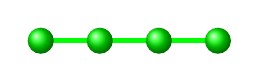
\begin{tikzpicture}[scale=0.75]
\tikzstyle{every node}=[ball color=green,circle,text=white]
\tikzstyle{edge from parent}=[draw,dashed,thick,green]
\draw[line width=2pt,color=green] (0,0) -- (1.0,0.0) -- (2.0, 0.0) -- (3.0, 0.0);
\node at (0,0) {};
\node at (1,0) {};
\node at (2,0) {};
\node at (3,0) {};
\end{tikzpicture}
\end{column}
\end{columns}
\end{frame}

\begin{frame}
\frametitle{Functions - Summary}
\begin{itemize}
\item Functions need to be declared before they are used. This is often done in \emph{header files}.
\item Up to one value can be returned from a function using the \kw{\tt return} statement.
\item A variable {\tt var} can be changed by a function if we pass the pointer
{\tt \&var}.
\item Pointers are declared using {\tt type * variable;}
\end{itemize}
\end{frame}

{
\setbeamercolor{frametitle}{bg=red}
\begin{frame}
\frametitle{Pointers II}
\begin{block}{Reminder}
\begin{itemize}
\item Declared using: {\tt type * ptrVar;}
\item Variable to pointer (pointer \emph{referencing}): {\tt ptrA = \&A;}
\item Pointer to variable (pointer \emph{de-referencing}):\\ {\tt *ptrA = newVar;}
\end{itemize}
\end{block}

\begin{exampleblock}{In addition}
Pointers are memory addresses, and as such allow arithmetic!
\end{exampleblock}
\end{frame}
}

\begin{frame}[fragile]
\frametitle{Variable sizes}
\begin{itemize}
\item Different data types take up different amounts of memory.
\item Example \kw{\tt float} is smaller than \kw{\tt double}.
\item The \kw{\tt sizeof} keyword gives a type's size (in bytes).
\end{itemize}

{
\small
\begin{semiverbatim}
\kw{\#include} \kt{<stdio.h>}

\kw{int} main()
\{
   printf(\kt{"sizeof(float) = \%d\\n"}, \kw{sizeof}(\kw{float}));
   printf(\kt{"sizeof(double) = \%d\\n"}, \kw{sizeof}(\kw{double}));
   printf(\kt{"sizeof(int) = \%d\\n"}, \kw{sizeof}(\kw{int}));
   printf(\kt{"sizeof(short) = \%d\\n"}, \kw{sizeof}(\kw{short}));
   \kw{return} 0;
\}
\end{semiverbatim}
}
\end{frame}

\begin{frame}
\frametitle{Arrays}
\begin{itemize}
\item These are blocks of data, all of the same type. Each element is indexed
using the array index operator:\\
e.g. {\tt myArray[index]} or {\tt primes[3]}.
\item Arrays are declared with types and sizes:\\
e.g. {\tt \kw{double} xVector[3];}
\item Arrays can be initialised:\\
e.g. {\tt \kw{int} primes[6] = \{2, 3, 5, 7, 11, 13\};}
\item All the elements of an array can be initialised to the \emph{same} value:
e.g. {\tt \kw{double} lotsOfDoubles[100] = \{0.0\};}
\item \bf Arrays in C are indexed from 0!
\end{itemize}
\end{frame}

\begin{frame}[fragile]
\frametitle{Accessing Array Elements}
\begin{alertblock}{}
\begin{center}
\bf Arrays in C are indexed from 0!
\end{center}
\end{alertblock}
\begin{semiverbatim}
\kw{\#include} \kt{<stdio.h>}

\kw{int} main()
\{
   \kw{int} primes[6] = \{2, 3, 5, 7, 11, 13\};

   printf(\kt{"first prime = \%d\\n"}, primes[0]);
   printf(\kt{"next prime = \%d\\n"}, primes[1]);
   
   \kw{return} 0;   
\}
\end{semiverbatim}
\end{frame}

{
\setbeamercolor{frametitle}{bg=red}
\begin{frame}[fragile]
\frametitle{Pointer Arithmetic}
\begin{itemize}
\item Different data types in C are different sizes.
\item Pointers are usually declared with a type (i.e. {\tt \kw{int} *},
{\tt \kw{float} *}, {\tt \kw{double} *}).


\begin{alertblock}{Relation to Arrays}
Given the array {\tt myArray} and an integer {\tt index}, the following is true:
\begin{center}
\tt myArray[index] = *(myArray + index)
\end{center}
\end{alertblock}

\item And this is the reason array indices start at 0...
\end{itemize}

\end{frame}
}

\begin{frame}
\frametitle{Debugging}
\begin{itemize}
\item Once you've designed, typed up and successfully compiled your program, the difficult part begins! Debugging!
\item Problems in the code are usually either easy to locate or stubbornly elusive.
\end{itemize}

\begin{exampleblock}{Easier Problems}
\begin{itemize}
\item Program crash/fault at the same point every run.
\end{itemize}
\end{exampleblock}

\begin{alertblock}{Nastier Problems}
\begin{itemize}
\item Numerical output differs to what is expected.
\item Program crashes seemingly randomly.
\end{itemize}
\end{alertblock}
\end{frame}

\begin{frame}
\frametitle{Debugging Techniques}
In increasing order of difficulty:
\begin{block}{Create Verbose Output}
\begin{itemize}
\item A few strategically placed {\tt printf} statements can prove to be helpful, but they are human readable:
\begin{itemize}
\item too few and you miss the problem,
\item too many and they rapidly become useless.
\end{itemize}
\item Straightforward to implement (and to comment out).
\end{itemize}
\end{block}

\begin{block}{Code Defensively}
\begin{itemize}
\item Consider specialised test cases.
\item Write code to test intermediate results.
\item Use the {\tt assert} macro.
\end{itemize}
\end{block}

\begin{block}{Use a Debugger}
For those non-trivial problems.
\end{block}
\end{frame}

\begin{frame}
\frametitle{Assertion Checking}
In the header \kt{\tt <assert.h>}, the macro {\tt assert} is defined. It has the following syntax:\\
\begin{center}
\tt assert(\emph{logical\_expression});
\end{center}
If \emph{logical\_expression} evaluates to false (zero) then:
\begin{itemize}
\item Program execution stops immediately.
\item An error message is sent to \emph{stderr} (the console) stating the line number where the assertion failed.
\end{itemize} 
\begin{block}{}
{\tt assert( a != 0); \kc{/* a should never be zero */}}
\end{block}
\begin{exampleblock}{Switching it off}
Placing {\tt \kw{\#define} NDEBUG} before all the \mbox{\tt \kw{\#include} \kt{<assert.h>}}
statements de-activates assertion checking.
\end{exampleblock}
\end{frame}

\begin{frame}[fragile]
\frametitle{Assertion Checking - An Example}
\vspace{-0.2in}
\begin{semiverbatim}
\scriptsize
\kr\kl\kw{\#include} \kt{<stdio.h>}
\kl\kw{\#include} \kt{<assert.h>}
\kl\kc{/* the sqrt function is much better than this... */}
\kl\kw{double} squareRoot(\kw{double} N)
\kl\{
\kl   \kw{double} x = 1.0;
\kl   \kw{int} loop;
\kl   \kc{/* negative numbers are not allowed! */}
\kl   assert(N >= 0.0);
\kl   \kw{if} (N == 0.0) \kw{return} 0.0;
\kl   \kw{for} (loop = 0; loop < 10; loop++)
\kl      x = (x*x+N)/(2.0*x);
\kl   \kw{return} x;
\kl\}
\kl
\kl\kw{int} main()
\kl\{
\kl   \kw{double} square;
\kl   printf(\kt{"Enter a non-negative number:"});
\kl   scanf(\kt{"\%lg"}, \&square);
\kl   \kc{/* SHOULD HAVE: if (x < 0.0) ...        */}
\kl   printf(\kt{"Square root = \%g\\n"}, squareRoot(square));
\kl   \kw{return} 0;
\kl\}
\end{semiverbatim}
\end{frame}

\begin{frame}
\frametitle{Using a Debugger}
\begin{itemize}
\item Two good debuggers are {\tt gdb} (GNU debugger) and Microsoft's Visual Studio debugger.
\item Programs need to be compiled with debug information.
\item Running a program straight through a debugger will show you the line of code that crashed it (if it crashes).
\end{itemize}

\begin{exampleblock}{Interactive Analysis of Running Code}
\begin{itemize}
\item Program execution can be paused at \emph{breakpoints}.
\item Functions can be \emph{stepped into}, \emph{stepped over}, or
\emph{stepped out from}.
\item Variables/arrays can be \emph{watched}.
\end{itemize}
\end{exampleblock}

\begin{alertblock}{}
Debuggers are very tricky to use at first, but can help isolate some very subtle problems.
\end{alertblock}
\end{frame}

\begin{frame}
\frametitle{Floating Point Numbers (IEEE 754 Standard)}
\framesubtitle{(from the previous lecture)}
On my machine, a \kw{\tt float} (single precision) looks like:\\
\begin{center}
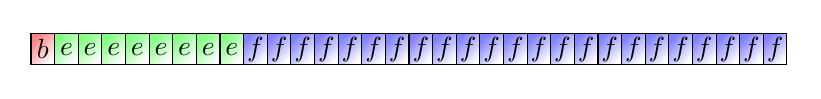
\begin{tikzpicture}[]
\shadedraw [top color=red!50,shading angle=45] (0,0) rectangle +(0.3,0.4);
\node at (0.15,0.2) {$b$};
\foreach \x in {0.3, 0.6, ..., 2.7}
   \shadedraw [top color=green!50,shading angle=45] (\x,0) rectangle +(0.3,0.4);

\foreach \x in {0.45, 0.75, ..., 2.85}
   \node at (\x,0.2) {$e$};
   
\foreach \x in {2.7, 3.0, ..., 9.6}
   \shadedraw [top color=blue!50,shading angle=45] (\x,0) rectangle +(0.3,0.4);
   
\foreach \x in {2.85, 3.15, ..., 9.45}   
   \node at (\x,0.2) {$f$};
\end{tikzpicture}
\end{center}
It consists of three parts, the \textcolor{red}{\emph{sign bit}$(b)$}, the \textcolor{green}{\emph{biased exponent}$(e)$} and the \textcolor{blue}{\emph{fraction}$(f)$}.
We break down a number $x$:
$$x^{\textrm{float}} = \textcolor{red}{(-1)^b} \times 
\textcolor{green}{2^{e-127}} \times \textcolor{blue}{\left(1+f\times2^{-23}\right)},
\begin{array}{c}
0 < e < 255\\0 \leq f \leq 2^{23}-1
\end{array},$$
We have three special numbers, {\tt -Inf} ($-\infty$), {\tt Inf} ($\infty$) and {\tt NaN} (Not a Number).

For \kw{\tt double} (double precision) we have:
$$x^{\textrm{double}} = (-1)^b\times 2^{e-1023}\times\left(1+f\times2^{-52}\right),
\begin{array}{c}
0 < e < 2047\\0 \leq f \leq 2^{52}-1
\end{array}.$$
\end{frame}

\begin{frame}
\frametitle{Floating Point Number Analysis}
In \kt{\tt <float.h>}, there are some useful quantities:
\resizebox{\textwidth}{!}{
\rowcolors[]{1}{blue!20}{blue!10}
\begin{tabular}{l l l}
\bf Quantity&\bf Float&\bf Double\\
Maximum Value&\tt FLT\_MAX&\tt DBL\_MAX\\
Minimum Value&\tt FLT\_MIN&\tt DBL\_MIN\\
Max Decimal Exponent&\tt FLT\_MAX\_10\_EXP&\tt DBL\_MAX\_10\_EXP\\
Min Decimal Exponent&\tt FLT\_MIN\_10\_EXP&\tt DBL\_MIN\_10\_EXP\\
$\epsilon$&\tt FLT\_EPSILON&\tt DBL\_EPSILON
\end{tabular}}

\begin{block}{Floating point $\epsilon$}
$\epsilon$ is the smallest (in magnitude) number such that:\\
\begin{center}
{\tt 1.0+$\epsilon$ != 1.0}
\end{center}
\end{block}
\end{frame}

\begin{frame}
\frametitle{Floating Point Accuracy}
\begin{itemize}
\item Some numbers can be represented in floating point exactly:
e.g. $2^i$, any integers that fit in the significand (mantissa).
\item Most numbers need to be approximated, e.g. $\sqrt{2}$, $\pi$.
\item One overlooked example is {\tt0.1}!
\item It is possible (though rare) to get exact answers from floating point arithmetic
\item Relative errors of $\approx10^{-15}$ for \kw{\tt double} and
$\approx10^{-6}$ for \kw{\tt float} are considered to be very good.
\item Multiplication and division generally preserve relative error (but can take us outside the floating point range).
\end{itemize}
\end{frame}

{
\setbeamercolor{frametitle}{bg=red}
\begin{frame}
\frametitle{The Largest Source of Floating Point Errors}
Addition and subtraction are the largest contributors to floating point error.

\begin{alertblock}{The Golden Rule}
{\bf Do not subtract two very similar floating point numbers!}
\end{alertblock}

(This leads to ``\emph{catastrophic cancellation}''.)
\end{frame}
}

\begin{frame}[fragile]
\frametitle{Casting}
Casting (the conversion of data from one type to another) can either be \emph{implicit} or \emph{explicit}.
\begin{block}{Implicit Casting}
Conversion where there is no ambiguity (i.e. to a ``bigger'' data type) can be done automatically:
\begin{semiverbatim}
\small\kw{double} x = 5; \kc{/* conversion from int to double */}
\kw{double} fEps = FLT_EPSILON; \kc{/* float to double */}
\end{semiverbatim}
\end{block}

\begin{block}{Explicit Casting}
If we wish to force a type conversion we place the destination type in brackets before the source variable:
\begin{semiverbatim}
oldtype oldData = ...
newtype newData = (newtype) oldData;
\end{semiverbatim}
Explicit casting should be avoided if possible.
\end{block}
\end{frame}

\begin{frame}
\frametitle{Scope: The Accessibility of Variables}
Every variable in C has, associated with it, a \emph{scope}. This defines how the variable can be accessed by functions in C. Some of the scoping rules are:
\begin{itemize}
\item All variables declared in the normal way inside a function are \emph{local} to that function.
\item Local variables can only be changed within the function they are defined,
\emph{unless}:
\begin{itemize}
\item A pointer to a local variable may be passed to a function, extending the scope of that variable.
\item The are declared to be {\tt extern} (more on this later).
\end{itemize}
\end{itemize}
\end{frame}

\begin{frame}[fragile]
\frametitle{Scope: Example 1}
\vspace{-0.1in}
\begin{semiverbatim}
\kr\kl\kw{\#include} \kt{<stdio.h>}
\kl
\kl\kw{void} F1()
\kl\{
\kl   \kw{int} i = 4;
\kl   printf(\kt{"In F1(): I = \%d\\n"}, i);
\kl\}
\kl
\kl\kw{int} main()
\kl\{
\kl   \kw{int} i = 2;
\kl   printf(\kt{"In main(): I = \%d\\n"}, i);
\kl   F1();
\kl   printf(\kt{"In main() again: I = \%d\\n"}, i);
\kl   \kw{return} 0;
\kl\}
\end{semiverbatim}
\end{frame}

\begin{frame}[fragile]
\frametitle{Scope: Example 2}
\vspace{-0.1in}
\begin{semiverbatim}
\kr\kl\kw{\#include} \kt{<stdio.h>}
\kl
\kl\kw{void} F1(\kw{int} i)
\kl\{
\kl   printf(\kt{"In F1(): I = \%d\\n"}, i);
\kl   i = 3;  \kc{/* what does this do? */}
\kl\}
\kl
\kl\kw{int} main()
\kl\{
\kl   \kw{int} i = 2;
\kl   printf(\kt{"In main(): I = \%d\\n"}, i);
\kl   F1(i);
\kl   printf(\kt{"In main() again: I = \%d\\n"}, i);
\kl   \kw{return} 0;
\kl\}
\end{semiverbatim}
\end{frame}

\begin{frame}[fragile]
\frametitle{Scope: Example 3}
\vspace{-0.1in}
\begin{semiverbatim}
\kr\kl\kw{\#include} \kt{<stdio.h>}
\kl
\kl\kw{void} F1(\kw{int} * i)
\kl\{
\kl   printf(\kt{"In F1(): I = \%d\\n"}, *i);
\kl   *i = 3;  \kc{/* what does this do? */}
\kl\}
\kl
\kl\kw{int} main()
\kl\{
\kl   \kw{int} i = 2;
\kl   printf(\kt{"In main(): I = \%d\\n"}, i);
\kl   F1(\&i);
\kl   printf(\kt{"In main() again: I = \%d\\n"}, i);
\kl   \kw{return} 0;
\kl\}
\end{semiverbatim}
\end{frame}

\begin{frame}[fragile]
\frametitle{Scope Blocks}
Variable scope is not restricted to functions, indeed anything contained in braces (\emph{scope blocks}) has it's own scope:
\vspace{-0.1in}
\begin{semiverbatim}
\small
\kr\kl\kw{\#include} \kt{<stdio.h>}
\kl
\kl\kw{int} main()
\kl\{
\kl   \kw{int} i = 1;
\kl
\kl   \kw{if} (i==1)
\kl   \{
\kl      \kw{int} j = 10; \kc{/* local to if block */}
\kl      printf(\kt{"i+j=\%d\\n"}, i+j);
\kl   \}
\kl
\kl   \kc{/* printf("j = \%d\\n", j); - error */}
\kl
\kl   \kw{return} 0;
\kl\}
\end{semiverbatim}
\end{frame}

\begin{frame}[fragile]
\frametitle{Local Variable Lifetime}
The lifetime of a local variable is limited:
\begin{semiverbatim}
\kw{\#include} \kt{<stdio.h>}

\kw{void} F1()
\{
   \kw{int} i = 1;
   printf(\kt{"In F1(): i = \%d\\n"}, i);
   i = i + 1; \kc{/* won't do much */}
\}

\kw{int} main()
\{
   F1();
   F1();
   \kw{return} 0;
\}
\end{semiverbatim}
\end{frame}

\begin{frame}
\frametitle{Local Variables}
\begin{itemize}
\item Every time {\tt F1()} is invoked, the value of {\tt i} is reset to 1.
\item The variable {\tt i} is a local variable which lives on the stack:
\begin{itemize}
\item it will be destroyed every time we leave {\tt F1()},
\item and recreated every time we invoke {\tt F1()}.
\end{itemize}
\item We can ask the C compiler to retain the value of {\tt i}:
\begin{block}{{\tt static} variables}
A variable can be declared to be \kw{\tt static}, this tells the C compiler to set aside memory other than the stack to store the variable. The variable will not be destroyed until the program ends.
\end{block}
\end{itemize}
\end{frame}

\begin{frame}
\frametitle{Why Use Static Variables?}
\begin{itemize}
\item To count the number of times a function has been called.
\item To have the function remember something between calls so on subsequent calls it can calculate what has changed (time, storage, the date, etc...), or resume from where it left off (reading from a list...)
\end{itemize}

\begin{exampleblock}{Worked Example: Elapsed Time}
\begin{itemize}
\item We write a function {\tt timer} which returns the time since it was last called.
\item Our program will contain two {\tt .c} files to demonstrate linking.
\end{itemize}
\end{exampleblock}
\end{frame}

\begin{frame}[fragile]
\frametitle{Timer Example: {\tt timer()}}
\begin{semiverbatim}
\kr\kl\kw{\#include} \kt{<time.h>} \kc{/* for clock function */}
\kl
\kl\kw{double} timer()
\kl\{
\kl   \kw{static double} oldTime = 0.0;
\kl   \kw{double} newTime, diff;
\kl
\kl   newTime = clock();
\kl   diff = newTime - oldTime;
\kl   oldTime = newTime;
\kl   \kw{return} diff/CLOCKS_PER_SEC;
\kl\}
\end{semiverbatim}
\end{frame}

\begin{frame}[fragile]
\frametitle{Timer Example: {\tt main()}}
\begin{semiverbatim}
\small
\kr\kl\kw{\#include} \kt{<stdio.h>}
\kl
\kl\kw{double} timer(); \kc{/* declare timer */}
\kl
\kl\kw{int} main()
\kl\{
\kl   timer(); \kc{/* reset clock */}
\kl   printf(\kt{"Wait... and hit return\\n"});
\kl   getchar(); \kc{/* wait for return */}
\kl   printf(\kt{"Elapsed time: \%.2f seconds\\n"}, timer());
\kl   printf(\kt{"Resetting clock, hit enter again\\n"});
\kl   getchar();
\kl   printf(\kt{"Elapsed time: \%.2f seconds\\n"}, timer());
\kl   \kw{return} 0;
\kl\}
\end{semiverbatim}
\end{frame}

\begin{frame}[fragile]
\frametitle{Global Variables - Shared between Functions}
We can define a \emph{global} variable:
\begin{semiverbatim}
\small
\kr\kl\kw{\#include} \kt{<stdio.h>}
\kl
\kl\kw{double} global = 42.0;
\kl
\kl\kw{void} F1()
\kl\{
\kl   printf(\kt{"Global = \%g\\n"}, global);
\kl\}
\kl
\kl\kw{int} main()
\kl\{
\kl   F1();
\kl   global = global + 1.0;
\kl   F1();
\kl   \kw{return} 0;
\kl\}
\end{semiverbatim}
\end{frame}

\begin{frame}
\frametitle{Global Variables - Between Multiple Files}
\begin{exampleblock}{Global to All Files}
If we want to share a global variable between files,
then we define it \emph{once} as:\\
{\tt type myglobalvariable = value;}\\
Then in every other file we declare it as:\\
{\tt \kw{extern} type myglobalvariable;}
\end{exampleblock}

\begin{alertblock}{Global Only to Current File}
If we do not wish to share a global variable, we
define it as follows:\\
{\tt \kw{static} type myPrivateGlobal = value;}
\end{alertblock}
\end{frame}

\begin{frame}[fragile]
\frametitle{Shared/Private Global Variables - File 1 of 2}
\begin{semiverbatim}
\footnotesize
\kr\kl\kw{\#include} \kt{<stdio.h>}
\kl
\kl\kw{int} globalEverywhere = 42;
\kl\kw{static int} globalHereOnly = 1;
\kl
\kl\kw{void} F2(); \kc{/* defined in file 2 */}
\kl
\kl\kw{int} main()
\kl\{
\kl   printf(\kt{"globalEverywhere = \%d\\n"}, globalEverywhere);
\kl   printf(\kt{"globalHereOnly = \%d\\n"}, globalHereOnly);
\kl
\kl   F2();
\kl
\kl   printf(\kt{"globalEverywhere = \%d\\n"}, globalEverywhere);
\kl   printf(\kt{"globalHereOnly = \%d\\n"}, globalHereOnly);
\kl
\kl   \kw{return} 0;
\kl\}
\end{semiverbatim}
\end{frame}

\begin{frame}[fragile]
\frametitle{Shared/Private Global Variables - File 2 of 2}
\vspace{-0.1in}
\begin{semiverbatim}
\small
\kr\kl\kw{\#include} \kt{<stdio.h>}
\kl
\kl\kw{extern int} globalEverywhere;
\kl\kc{/*if we forget the extern we get a linker error */}
\kl
\kl\kw{static int} globalHereOnly = 100;
\kl
\kl\kw{void} F2()
\kl\{
\kl   printf(\kt{"F2(): globalEverywhere = \%d\\n"},
\kl                 globalEverywhere);
\kl                 
\kl   printf(\kt{"F2(): globalHereOnly = \%d\\n"},
\kl                 globalHereOnly);
\kl\}
\end{semiverbatim}
\end{frame}

\begin{frame}
\frametitle{Imperative versus Functional Programming}
Two programming techniques are popular in C:
\begin{alertblock}{Imperative}
\begin{itemize}
\item Very long functions.
\item Lots of global variables.
\item Very few function calls.
\end{itemize}
\end{alertblock}

\begin{exampleblock}{Functional}
\begin{itemize}
\item Lots of small functions.
\item Each function has a clearly defined r\^ole.
\item Global variables avoided as much as possible.
\end{itemize}
\end{exampleblock}

I would encourage leaning towards the latter, a good program will contain traits from both styles.
\end{frame}

\begin{frame}[fragile]
\frametitle{The C Preprocessor - Conditional Compilation}
We have already seen the {\tt \kw{\#include}} statement. Conditional statements are also possible:
\vspace{-0.2in}
\begin{semiverbatim}
\small
\kr\kl\kw{\#include} \kt{<stdio.h>}
\kl
\kl\kw{int} main()
\kl\{
\kl\kw{\#ifdef} NDEBUG
\kl   printf(\kt{"Assertions DISABLED\\n"});
\kl\kw{\#else}
\kl   printf(\kt{"Assertions ENABLED\\n"});
\kl\kw{\#endif}
\kl   \kw{return} 0;
\kl\}
\end{semiverbatim}
\begin{alertblock}{}
This logic is performed at \emph{compile time}.
\end{alertblock}
\end{frame}

\begin{frame}
\frametitle{The C Preprocessor - How to {\tt\#define} Externally}
We are not restricted to {\tt \kw{\#define}} statements in source code.
\begin{block}{Visual Studio}
In the Visual Studio ``project properties'' $\rightarrow$ ``C/C++'' $\rightarrow$ ``Preprocessor'' option we can specify preprocessor definitions.
\end{block}

\begin{block}{gcc}
In gcc we can specify define statements in the command line as follows:\\
{\tt gcc myfile.c -DNDEBUG -o myprogram }
\end{block}
\end{frame}




\end{document}




